\chapter{Implementación}

	\section{¿Qué es una FPAA?}
	Una FPAA  por sus siglas en inglés (Field Programmable Analog Arrays) es un dispositivo analógico equivalente a las FPGA (Field Programmable Garte Arrays). A diferencia de las FPGA que contienen una gran cantidad de módulos y conexiones que permiten configuraciones arbitrarias de lógica combinacional y secuencial, los FPAA generalmente contienen una pequeña cantidad de CABs (Configurable Analog Blocks). Los FPAA dirigidos al diseño analógico estándar generalmente presentan un CAB que contiene un amplificador operacional, un arreglo de capacitores programables, y ya sea un arreglo de resistencias programables para circuitos en tiempo continuo o switches configurables para circuitos de capacitores conmutados.
	Se trabajó con la tarjeta Anadigm QuadApex Develovment Boarsd v2.0 de la empresa Anadigm, la cual contiene 4 FPAAs AN231E04 que pueden conectarse en cadena y es programada mediante el software AnadigmDesigner2 (AD2). El diagrama esquemático de la tarjeta se puede ver en la Figura \ref{fig:esquematico_fpaa} del apéndice.
	
	\section{Características de la tarjeta y requerimientos}
	
	\subsection{Alimentación de la tarjeta}
	Para el correcto funcionamiento de la placa esta debe ser alimentada con una fuente de voltaje regulada a 5V de al menos 500mA conectada a la clema de dos terminales. Hay un LED de color verde que indica que la placa se ha encendido correctamente, la placa esta protegida contra la conexión de una fuente de voltaje con la polarización incorrecta.
	
	\subsection{Instalación de drivers}

No conecte la placa QuadApex v2.0 a la PC vía cable USB,  ni tampoco inicie AD2 ahora, el driver debe instalarse primero. Se asume que AD2 ya ha sido instalado y registrado en su computadora, de lo contrario entre al link que aparece a continuación.

Para instalar AD2 basta con acceder al siguiente link y seguir los pasos que muestra la pagina:

	\begin{center}
		\url{https://www.anadigm.com/sup_downloadcenter.asp?tab=ad2}
	\end{center}

es recomendable guardar los datos de registro en un lugar seguro, al iniciar el programa por primera vez es necesario ingresar el \textbf{License ID} y la \textbf{License key} estos estarán en el correo que le proporcionó a Anadigm. 

El driver \textbf{CP210x\_{}Drivers.exe} está incluido en el AD2 CD o se puede encontrar en la página de Silicon Labs. Siga los siguientes pasos si es la primera vez que instala este driver, de lo contrario desinstale las versiones anteriores antes de continuar:

\begin{enumerate}
	\item Ejecute como administrador el ejecutable  CP210x\_{}Drivers.exe. El destino por defecto del ejecutable es ‘‘C:\textbackslash{}Silabs\textbackslash{}Mcu\textbackslash{}CP210x’’.
	\item Para completar la instalación conecte la QuadApex v2.0 y enciéndala.
	\item Acceda al administrador de dispositivos y en \textbf{Puertos (COM y LPT)} asegúrese que el driver este bien configurado, si no aparece un signo de admiración y se le asigno un puerto COM  la instalación fue exitosa, de lo contrario dar clic derecho sobre el dispositivo y seleccionar \textbf{Actualizar controlador}, después buscar el  driver en la ruta del paso 1.
\end{enumerate}

El driver en este punto ya esta instalado. La instalación del driver y la asignación del puerto es necesaria solo una vez. Si se conecta subsecuentemente a otro puerto de USB de la PC puede ser necesario repetir el paso 3.
	
	\subsection{Jumpers por defecto}
	
	En la Tabla \ref{tab:jumpers} se muestra una lista con los jumpers que contiene la placa, una descripción de su funcionamiento y su posición por defecto. Es importante colocar la FPAA con todos sus jumper en el estado por defecto para entender secciones posteriores y evitar errores. La placa no contiene una cantidad muy grande de jumpers y usualmente solo se modificarán los jumpers J8,9,10, los cuales son los que controlan la cantidad de FPPAs activas.
	
\begin{table}[!ht]
		\centering
		\caption{Resumen de jumper de la placa}
		\label{tab:jumpers}
		\resizebox{15cm}{!} {
		\begin{tabular}{|p{1.7cm}|p{9.5cm}|p{4.5cm}|p{5.5cm}|}
			\hline
			\textbf{Jumper} &  \textbf{Función} & \textbf{Estado por defecto}	& 	\textbf{Condición por defecto}\\
			\hline
			J1		&	Conecta la sección digital a la sección analógica.	&	Todos los 13 jumpers deben estar conectados &	Conecta completamente la alimentación, tierra y todas las señales digitales FPAA a la sección digital.\\
			\hline
			J2		&	Selecciona entre 16MHz y 40MHz para la fuente ACLK. &	Jumpers off &	ACLK$=$16MHz\\
			\hline
			J3		& Permite la descarga de la configuración de prueba a todos los FPAA desde FLASH (después de reiniciar o apagar y encender). El circuito de prueba despliega ondas sinusoidales a todas las salidas FPAA. &	Jumper off	& Descarga del circuito de prueba deshabilitado\\
			\hline
			J4		& Permite el almacenamiento de configuraciones primarias en el FLASH del PIC32 si el puente está activado. & Jumper off		&	No en modo de almacenamiento de configuraciones primarias.\\
			\hline
			J5		& Jumper de repuesto.	&	Jumper off &	-\\
			\hline
			J6		& Un jumper en J5 deshabilitará el módulo oscilador de 16MHz y tristateará su salida. Esto significa que el pin ACLK de los FPAA no se sincronizará, tampoco se sincronizará el microcontrolador PIC32, por lo que toda la placa se desactivará efectivamente. & Jumper off	& Oscilador de 16MHz habilitado	\\
			\hline
			J7		& Este jumper controla la generación de un suministro negativo (-3.3V) para las etapas del buffer de salida en la placa. El puente a la derecha desactiva el suministro negativo (lo ata al suelo). El puente a la izquierda permite el suministro.	& Jumper a la izquierda	&	Alimentación negativa habilitada\\
			\hline
			J8,9,10	& Estos jumpers en combinacion con ACT1, ACT2, ACT3, ACT4 controlan la cadena de FPAAs.	& Todos los jumpers especificados deben estar conectados	& Todas las FPAA en cadena	\\
			\hline
			J11		& Estos jumpers conectan el transceptor USB a la interfaz UART del microcontrolador PIC32. Si no se requiere control USB, estos 4 puentes se pueden quitar.	& Todos los jumpers conectados	& USB habilitado 	\\		
			\hline
		\end{tabular}
		}
\end{table}


	\subsection{Tamaño variable de cadena de FPAAs}

	La placa contiene 4 FPAAs en cadena. Esta cadena puede ser cortada a 3, 2 o 1, pero debe ser cortada deshabilitando FPAAs desde el final de la cadena (del lado derecho).

\begin{itemize}
	\item Pare reducir la cadena a 3 FPAAs, remueva los jumpers de \textbf{J10} y también el jumper marcado \textbf{ACT4} de \textbf{J1}. Esto deshabilitará FPPAA \#4 (la más cercana a la fuente de alimentación.)
	\item Para reducir la cadena a 2 FPAAs, remueva los jumpers de \textbf{J9} y \textbf{J10} y también los jumpers marcados \textbf{ACT3} y \textbf{ACT4} de \textbf{J1}. Esto deshablitará los FPAAs \#3 y \#4.
	\item Para reducir la cadena a 1 FPAA, remueva los jumpers de \textbf{J8, J9} y \textbf{J10} y  también los jumpers marcados \textbf{ACT2, ACT3} y \textbf{ACT4} de \textbf{J1}. Esto deshabilitará los FPAA \#2, \#3 y \#4.
\end{itemize}
\textbf{Nota:} si se configura una cadena de FPAA y luego se desconectan 1 o más FPAA de la cadena, los FPAA desconectados aún mantendrán su configuración hasta que se reinicie la placa o se vuelva a configurar la cadena (reducida).

	\subsection{DIP Switches}
	
	El usuario puede hacer sus propias conexiones en la placa con cables, pero hay un conjunto de DIP switches que permiten una fácil conexión de ciertas rutas entre los FPAA vecinos y entre los FPAA y los \textbf{input/output buffers}. Estos interruptores están abiertos por defecto, lo que significa que todos están hacia la izquierda. El usuario puede cerrar los interruptores empujándolos hacia la derecha. En la Tabla \ref{tab:switches} se muestra un resumen de los switches. Los DIP switches son pequeños y del tipo deslizantes, por lo que se recomienda una herramienta afilada como un destornillador delgado para abrir y cerrar los switches. Algunos ejemplos se muestran a continuación:
	
	\begin{enumerate}
		\item Para conectar el filtro Rauch\_\#1\_I01 a I1 de la FPPA\#{}1, cierre los 4 interruptores en S10.
		\item Para conectar O4 del FPAA\#{} a I1 del FPAA\#{}2, cierre los 2 interruptores superiores de S2.
		\item Para conectar O3 del FPAA\#{}1 al buffer de salida BUF\_\#1\_03, cierre ambos switches de S13.
	\end{enumerate}

	\begin{table}[!ht]
		\centering
		\begin{tabular}{|l|l|l|}
			\hline
			\textbf{Función} &  \textbf{Tipo} & \textbf{Labels}\\
			\hline
			Conectar filtros Rauch a entradas de FPAA 					& 4way 		& S8,9,10,11,15,16,17,18		\\
			\hline
			Conectar entre FPAAs 						& 4way 	& S2,3,4,5,6,7	\\
			\hline
			Conectar FPAA a buffers de salida 						& 2way 		& S12,13,14,19		\\
			\hline
		\end{tabular}
		\caption{DIP Switches}
		\label{tab:switches}
	\end{table}

	\subsection{Filtros Rauch y buffers de salida}
	
	La tarjeta cuenta con 2 buffers de entrada llamados filtros Rauch listos para usar, \textbf{Rauch\_\#1\_I01} y \textbf{Rauch\_\#2\_I01}, estos son filtros multipropósito cuya su principal función es convertir una señal single-ended a una diferencial en la FPAA, internamente la FPAA trabaja únicamente con señales diferenciales y debido a esto el uso de estos filtros es imprescindibles para introducir señales externas, por ejemplo de generadores de funciones u otros circuitos. Si se usa una señal single-ended, es necesario conectar IN- a GND y conectar la señal en IN+.
	Para activar el filtro es necesario hacerlo desde el software AD2 haciendo doble clic en la IO cell apropiada (IOCell1-4), seleccionar Input y después Amplifier, esto es debido a que el filtro funciona en combinación con un amplificador integrado en la FPAA y los componentes pasivos de montaje superficial que vienen soldados de fabrica.
	
	Rauch\_\#1\_I01 está conectado a I/O1 de la FPAA \#1 y esta configurado con una frecuencia de corte muy alta y ganancia unitaria ($F_{o} = 490$KHz). Rauch\_\#21\_I01 está conectado a I/O1 de la FPAA \#2 y esta configurado con una ganancia unitaria y una frecuencia de corte de poco más de 20kHz, que es típica de una aplicación de audio. 

	La tarjeta también cuenta con 2 buffers de salida listos para usar, \textbf{Buf\_\#1\_O3} y  \textbf{Buf\_\#2\_O3}, cuyo principal propósito es convertir la salida diferencial de la FPAA a una single-end. 
	Buf\_\#1\_O3 está conectado a O3 de la FPAA \#1 y está configurado con una frecuencia de corte muy alta y una ganancia unitaria. Si se requiere una frecuencia de corte inferior, es muy fácil modificar este filtro sin quitar los componentes de montaje superficial debajo, simplemente agregando capacitores TH. Buf\_\#2\_O3 está conectado a O3 de FPAA \#2 y esta configurado con una ganancia unitaria y una frecuencia de corte de poco más de 20 kHz, que es típica de una aplicación de audio. 
	
	Cabe resaltar que para utilizar tanto los filtros Rauch como los buffers de salida sin cables adicionales es necesario cerrar los DIP switches correspondientes, no obstante se pueden cablear externamente a cualquiera de las entradas o salidas de las FPAA.
	
	\subsection{Circuito de prueba}

La placa es capaz de autoconfigurar los FPAAs con un circuito de prueba para una verificación rápida de la placa. Para hacer esto, coloque un jumper en \textbf{J3} y reinicie la placa. Todos los FPAA en la cadena ahora se configurarán con el circuito de prueba (el LED verde indica que la configuración fue exitosa). Este circuito de prueba genera una onda sinusoidal en todas las 7 salidas del FPAA (14 salidas diferenciales). La frecuencia de esta onda sinusoidal es de 1kHz en FPAA \#{}1, 2kHz en FPAA \#{}2, 4kHz en FPAA \#{}3 y 8kHz en FPAA \#{}4. Si se habilitan menos de 4 FPAA en la cadena, solo se configurarán aquellos FPAA que estén habilitados. Si se coloca un jumper en \textbf{J3} y \textbf{J4}, se cargará un circuito diferente en los FPAAs. Este es un circuito de prueba especial utilizado por Anadigm durante la producción. Se aconseja al usuario que no coloque jumpers en J3 y J4 al mismo tiempo.

	\section{AnadigmDesigner2}
	
	AD2 trabaja con módulos llamados CAMs (Configurable Analog Modules), estos aportan flexibilidad y sencillez en el proceso diseño debido a que son bloques que hacen desde funciones sencillas como inversores o comparadores hasta diseños completos como filtros y multiplicadores, los CAMs se pueden interconectarse fácilmente unos con otros y únicamente necesitan pequeñas configuraciones para su correcto funcionamiento. Los CAMs más utilizados en el diseño de osciladores caóticos son los mostrados en la Tabla \ref{tab:CAMs_AD2}.
	

\begin{table}[!ht]
  \centering
  \caption{CAMs básicos de AD2}
  \label{tab:CAMs_AD2}
  \begin{tabular}{>{\centering\arraybackslash}m{3cm} >{\centering\arraybackslash}m{5cm} >{\centering\arraybackslash}m{5cm}}
    \hline
    \textbf{Nombre} & \textbf{Función de transferencia} & \textbf{Descripción}\\ 
    \hline
    {\scriptsize \textbf{GainInv}}
    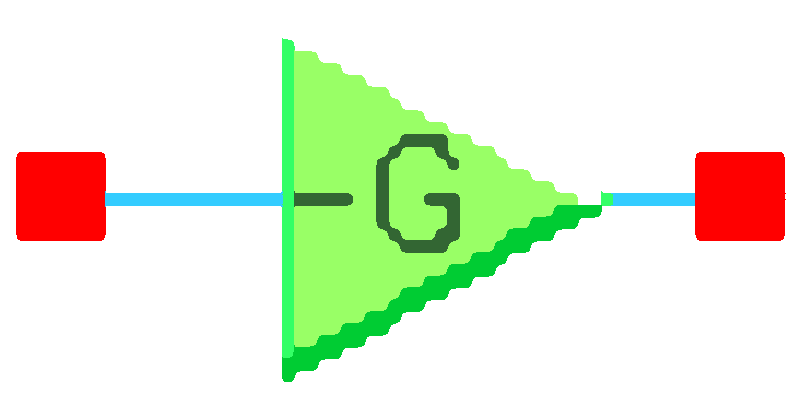
\includegraphics[width=2.2cm]{T7_Inversor.eps}
    &
      $\frac{V_{\mathrm{out}} (s)}{V_{\mathrm{in}}(s)} = - G$
    & 
      \begin{itemize}[leftmargin=0cm,noitemsep]
      \begin{scriptsize}
		\item[] Ganancia inversora.
		\item[] Gain: 0.01 - 100.0 V/V
      \end{scriptsize}
      \end{itemize}
    \\ %-------------------------------------------------------
    {\scriptsize \textbf{Integrator}}
    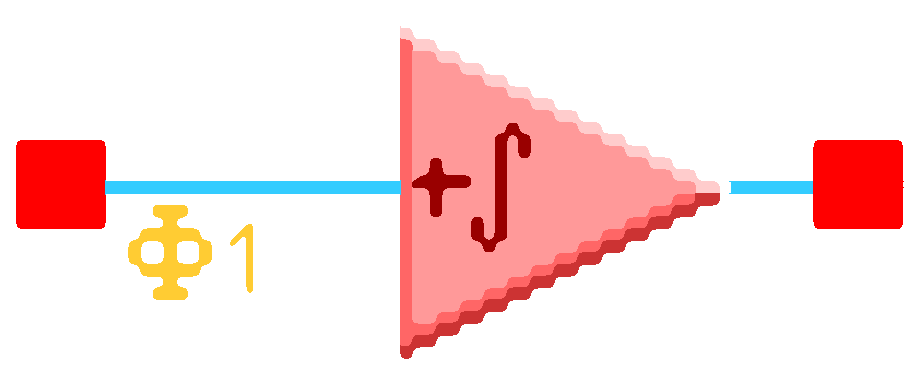
\includegraphics[width=2.5cm]{T1_Integrador.eps}
    &
      $ \frac{V_{\mathrm{out}} (s)}{V_{\mathrm{in}}(s)} = \frac{\pm K}{s}$
    & 
      \begin{itemize}[leftmargin=0cm,noitemsep]
      \begin{scriptsize}
		\item[] Integrador con una constante de integración programable. La salida puede ser inversora o no inversora.
      \end{scriptsize}
      \end{itemize}
    \\ %-------------------------------------------------------
    {\scriptsize \textbf{Voltage}} \linebreak
    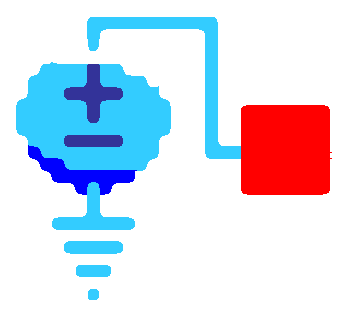
\includegraphics[width=1cm]{T6_DC_voltage.eps}
    &
      $V_{\mathrm{out}} = \pm 2$
    & 
      \begin{itemize}[leftmargin=0cm,noitemsep]
      \begin{scriptsize}
		\item[] Referencia de voltaje de $\pm$ 2 V.
      \end{scriptsize}
      \end{itemize}
    \\ %-------------------------------------------------------
    {\scriptsize \textbf{TransferFunction}} \linebreak
    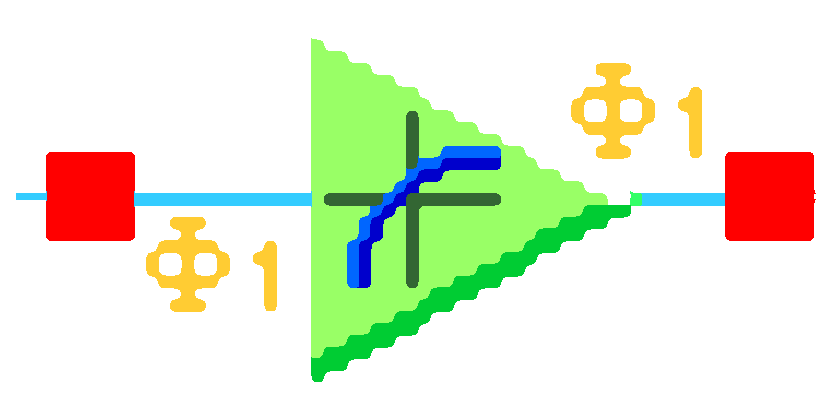
\includegraphics[width=2.5cm]{T3_Transferfunction.eps}
    &
    & 
      \begin{itemize}[leftmargin=0cm,noitemsep]
      \begin{scriptsize}
		\item[] \textbf{Lookup Table}: función de transferencia especificada por el usuario de 256 de pasos de cuantificación.  
      \end{scriptsize}
      \end{itemize}
    \\ %-------------------------------------------------------
    {\scriptsize \textbf{Multiplier}} \linebreak
    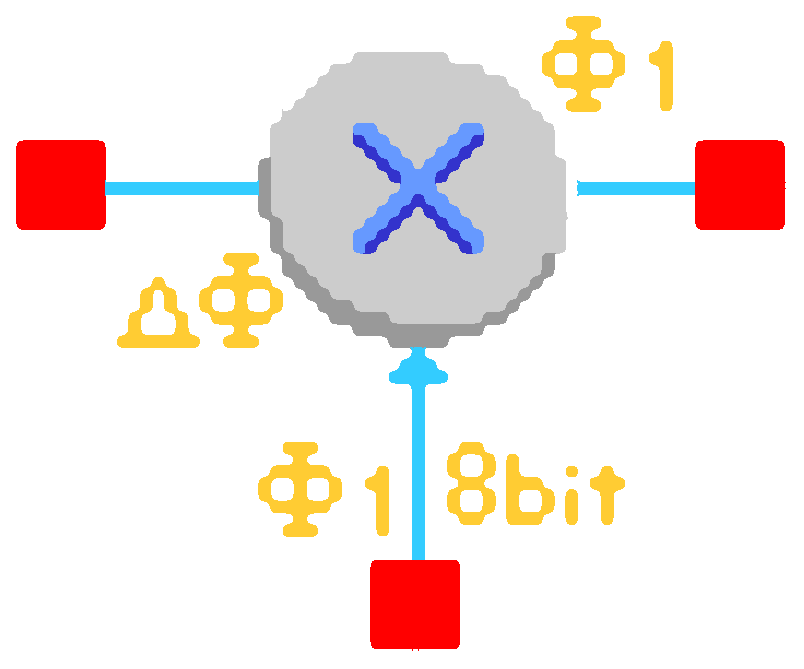
\includegraphics[width=2.5cm]{T2_Multiplicador.eps}
    &
      $V_{\mathrm{out}} = M \cdot V_{x} \cdot V_{y}$
    & 
      \begin{itemize}[leftmargin=0cm,noitemsep]
      \begin{scriptsize}
		\item[] $V_{x}$ es la entrada de voltaje izquierda.
		\item[] $V_{y}$ es la entrada de voltaje inferior cuantificado de 8 bits.
		\vspace{-0.15cm}
		\item[] $M$ factor de multiplicación.
      \end{scriptsize}
      \end{itemize}
    \\ %-------------------------------------------------------
    {\scriptsize \textbf{SumDiff}} \linebreak
    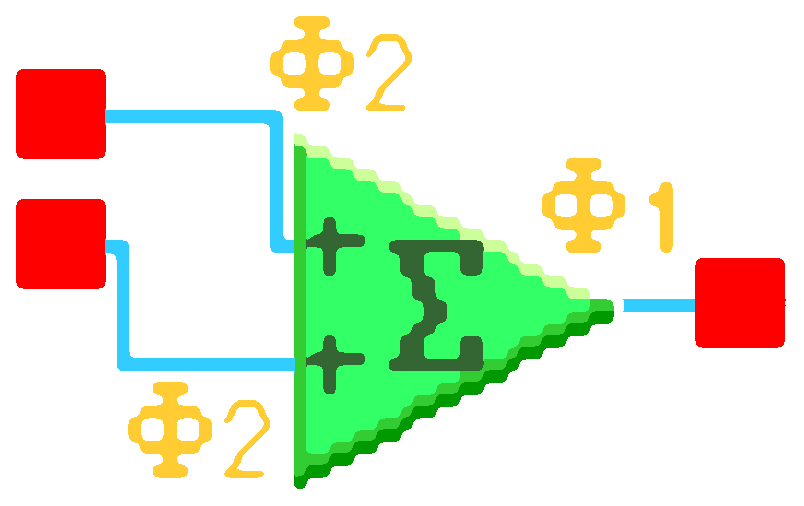
\includegraphics[width=2.5cm]{T8_Sumador.eps}
    &
      \begin{footnotesize}
      	$V_{\mathrm{out}} = \pm G_{1} V_{\mathrm{in1}} \pm G_{2} V_{\mathrm{in2}} \pm G_{3} V_{\mathrm{in3}} \pm G_{4} V_{\mathrm{in4}}$
      \end{footnotesize}
    & 
      \begin{itemize}[leftmargin=0cm,noitemsep]
      \begin{scriptsize}
		\item[] Las entradas pueden ser inversoras o no inversoras.
		\item[]	Cada entrada tiene una ganancia programable.
		\vspace{-0.15cm}
		\item[] Configurable desde 2 hasta 4 entradas. 
      \end{scriptsize}
      \end{itemize}
    \\ %-------------------------------------------------------
    {\scriptsize \textbf{FilterBilinear}} \linebreak
    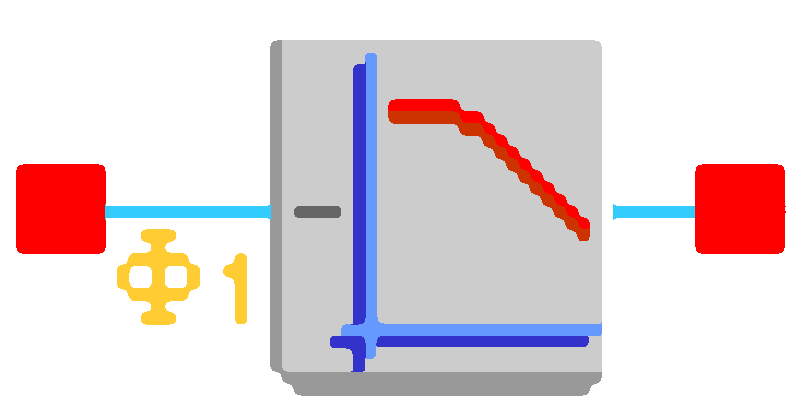
\includegraphics[width=2.5cm]{T9_FilterBilinear.eps}
    &
      \begin{scriptsize}
		 \textbf{Low Pass Bilinear Filter} \linebreak
      	 $\frac{V_{\mathrm{out}}(s)}{V_{\mathrm{in}}(s)} = \pm \frac{2 \pi f_{0} G}{s + 2 \pi f_{0}}$ \linebreak
      	 \textbf{High Pass Bilinear Filter} \linebreak
      	 $\frac{V_{\mathrm{out}}(s)}{V_{\mathrm{in}}(s)} = - \frac{Gs}{s + 2 \pi f_{0}}$ \linebreak
      	 $\vdots$
      \end{scriptsize}
    & 
      \begin{itemize}[leftmargin=0cm,noitemsep]
      \begin{scriptsize}
		\item[] Puede ser configurado como pasabajas, pasaaltas, pasatodas o general (Polo y cero).
      \end{scriptsize}
      \end{itemize}
    \\ %-------------------------------------------------------
    {\scriptsize \textbf{FilterBiquad}} \linebreak
    \includegraphics[width=2.5cm]{T10_FilterBiquad.eps}
    &
      \begin{scriptsize}
		 \textbf{Low Pass Biquadratic Filter} \linebreak
      	 $\frac{V_{\mathrm{out}}(s)}{V_{\mathrm{in}}(s)} = \frac{\pm 4 \pi^{2} f_{0}^{2} G}{s^{2} + \frac{2 \pi f_{0}}{Q}s + 4 \pi^{2} f_{0}^{2}}$ \linebreak
      	 \textbf{High Pass Biquadratic Filter} \linebreak
      	 $\frac{V_{\mathrm{out}}(s)}{V_{\mathrm{in}}(s)} = \frac{-G s^{2}}{s^{2} + \frac{2 \pi f_{0}}{Q} s + 4 \pi^{2} f_{0}^{2}}$ \linebreak
      	 $\vdots$
      \end{scriptsize}
    & 
      \begin{itemize}[leftmargin=0cm,noitemsep]
      \begin{scriptsize}
		\item[] Puede ser configurado como pasabajas, pasaaltas, pasabanda, rechazabanda o general (Polos y ceros).
      \end{scriptsize}
      \end{itemize}
    \\ %-------------------------------------------------------
    \hline
  \end{tabular}
\end{table}

	Las configuraciones de los CAMs dependen de las frecuencias de reloj que se seleccionen para cada FPAA. Cada FPAA tiene dos fuentes de frecuencias de reloj principales \textbf{Sys1} y \textbf{Sys2}, y cinco frecuencias de reloj de chip, desde \textbf{Clock 0} hasta \textbf{Clock 5} que son subdivisiones de cualquiera de las fuentes de reloj principales. Seleccionar y configurar correctamente los relojes es importante ya que el rango de operación de los CAMs depende de esto. 

	\section{Implementación con aproximación de primer orden}
	
	Para realizar la implementación física de la aproximación de primer orden del integrador fraccionario se utilizó el CAM \textbf{FilterBilinear} en su modo \textbf{Pole and Zero}, esto debido a su flexibilidad y semejanza con la función de transferencia de la aproximación de la CFE de primer orden. La función de transferencia del CAM en este modo es la siguiente:
	
	\begin{equation}
		\frac{V_{\mathrm{out}} (s)}{V_{\mathrm{in}}(s)} = -\frac{G_{H} (s + 2 \pi f_{z})}{s + 2 \pi f_{p}}
	\end{equation}
	donde $G_{L}$ esta definida como:
	\begin{equation}
		G_{L} = \frac{f_{z}}{f_{p}} G_{H}
	\end{equation}
	y donde $G_{L}$ es la ganancia en DC, $G_{H}$ es la ganancia de alta frecuencia, $f_{p}$ es la frecuencia del polo y $f_{z}$ es la frecuencia del cero.
	
	La función de transferencia de la aproximación con la CFE de primer orden, como se mencionó anteriormente es la siguiente:
	\begin{equation}
		\genfrac{}{}{0pt}{0}{}{_{(c_{2})}} \frac{1}{s^{\alpha}} \approx \frac{(1 - \alpha)s + (1 + \alpha) }{(1 + \alpha)s + (1 - \alpha)} 
		\label{ec:cfe_primer_orden}
	\end{equation}
	si consideramos la siguiente sustitución:
	
	\begin{equation}
		A = \frac{1 - \alpha}{1 + \alpha}
	\end{equation}
	podemos reescribir la ecuación (\ref{ec:cfe_primer_orden}) de la siguiente manera:
	
	\begin{equation}
		\genfrac{}{}{0pt}{0}{}{_{(c_{2})}} \frac{1}{s^{\alpha}} \approx \frac{A s + 1}{s + A}
		\label{ec:cfe_primer_orden_simp}
	\end{equation}
	aplicando el escalamiento en frecuencia a la ecuación (\ref{ec:cfe_primer_orden_simp}) se convierte en:
	
	\begin{equation}
		\frac{A s + k_{f}}{s + A k_{f}}
		\label{ec:cfe_primer_orden_simp_esc}
	\end{equation}
	
	Esto es una prueba 